%!LW recipe=pdfLaTeXmk

\documentclass[scheme=plain]{beamer}
\usepackage[T1]{fontenc}
\usepackage{fontawesome5}
\usepackage{mathtools}
\usepackage{tikz}
\usepackage{booktabs}
\usepackage{caption}
\usepackage{outlines}
\usepackage{graphicx}
\usepackage{float}
\usepackage{amsthm}
\usepackage{tabularray}
\usepackage{minted}
\usepackage{hyperref}
\usepackage{cleveref}
\usepackage{url}
\usepackage{xspace}
\usepackage{academicons}
\usepackage{pgfplots}
\usepackage{pgfgantt}
\usepackage{qrcode}
\usepackage{ninecolors}
\usepackage{soul}
\usepackage[style=numeric, backend=biber, url=false, doi=false, isbn=false]{biblatex}
\newmintinline[code]{html}{fontsize=\small}
\addbibresource{yuxuan.bib}
\usepackage{graphicx}
\usetheme[
    progressbar=frametitle,
    numbering=fraction,
    subsectionpage=progressbar,
    titleformat title=smallcaps,
    titleformat subtitle=smallcaps,
    titleformat section=smallcaps,
    titleformat frame=smallcaps]{moloch}

    
\setbeamercolor{palette primary}{bg=gray1}
\setbeamercolor{frametitle}{bg=black,fg=white}
\setbeamercolor{progress bar}{fg=black}
\setbeamerfont{footnote}{size=\tiny}
\renewcommand{\cite}{\footfullcite}

\usetikzlibrary{calc}
\setcounter{tocdepth}{1}

\makeatletter
\newlength{\frametitle@padding}
\setlength{\frametitle@padding}{2.2ex}
\newcommand{\frametitlestrut@start}{
  \rule{0pt}{\frametitle@padding +%
    \totalheightof{%
      \ifcsdef{frametitleformat}{\frametitleformat X}{X}%
    }%
  }%
}

\newcommand{\frametitlestrut@end}{
  \rule[-\frametitle@padding]{0pt}{\frametitle@padding}
}

\setbeamertemplate{frametitle}{
    \nointerlineskip%
    \begin{beamercolorbox}[%
        wd=\paperwidth,%
        sep=0pt,%
        leftskip=\frametitle@padding,%
        rightskip=\frametitle@padding,%
      ]{frametitle}%
    \frametitlestrut@start%
    \insertframetitle%
    \hfill%
    \nolinebreak%
    \frametitlestrut@end%
    \end{beamercolorbox}%
    % \begin{tikzpicture}[remember picture,overlay]
    %     \coordinate (logo) at ([xshift=-1.8cm,yshift=-0.5cm]current page.north east);
    %     \node at (logo) {\includegraphics[height=.1\textheight]{northeastern.eps}};
    % \end{tikzpicture}
}
\makeatother


\setbeamertemplate{footline}{
    \hbox{%
    \begin{beamercolorbox}[wd=\paperwidth,ht=3ex,dp=1.5ex,leftskip=2ex,rightskip=2ex]{page footer}%
        \usebeamerfont{title in head/foot}%
        \hfill
        \begin{tblr}{
            width=.8\linewidth,
            colspec={X[l]X[c]X[r]}
        }
            \insertsectionhead{}
            &
            \ifx\insertsubsection\empty
            \else
            \insertsubsection{} 
            \fi
            &
            \insertframenumber{} / \inserttotalframenumber
        \end{tblr}
        \hfill{}
    \end{beamercolorbox}}%
}

\defbeamertemplate{section page}{my progressbar}{
  \centering
  \begin{minipage}{22em}
    \raggedright
    \usebeamercolor[fg]{section title}
    \usebeamerfont{section title}
    \insertsection\\[-1ex]
    \usebeamertemplate*{progress bar in section page}
    \par
    \ifx\insertsubsectionhead\@empty\else%
      \usebeamercolor[fg]{subsection title}%
      \usebeamerfont{subsection title}%
      \insertsubsectionhead
    \fi
  \end{minipage}
  \par
  \vspace{\baselineskip}
}
\setbeamertemplate{section page}[my progressbar]


\UseTblrLibrary{booktabs}
\graphicspath{ {./figures/} }

\title{UXAgent: A System for Simulating Usability Testing of Web Design with LLM Agents}

\author{\textbf{Yuxuan Lu\textsuperscript{1,2}},
\textbf{Bingsheng Yao\textsuperscript{2}},
\textbf{Hansu Gu\textsuperscript{1}},
\textbf{Jing Huang\textsuperscript{1}},
\textbf{Zheshen (Jessie) Wang\textsuperscript{1}},
\textbf{Yang Li\textsuperscript{1}},
\textbf{Jiri Gesi\textsuperscript{1}},
\textbf{Qi He\textsuperscript{1}},
\textbf{Toby Jia-Jun Li\textsuperscript{3}},
\textbf{Dakuo Wang\textsuperscript{1,2}}}

\institute{\textsuperscript{1}Amazon.com, Inc.,
\textsuperscript{2}Northeastern University,
\textsuperscript{3} University of Notre Dame}
\date{Dec 1, 2025}
\begin{document}

\maketitle


\begin{frame}{What’s the worst nightmare as a researcher?}
  \begin{outline}
    \1 The myth of “Review 2”
    \1 Paper being scooped
    \1 Realizing that your experiment design is flawed one week before deadline
  \end{outline}
\end{frame}

\begin{frame}{As someone from both NLP and HCI, I think …}
\begin{table}
  \centering
  \begin{booktabs}{
    colspec = {X[c]X[c]X[c]},
    width = \linewidth,
    cells={m},
  }
  \toprule
  Field & NLP & HCI \\
  \midrule
  Experiment Subject & Models and Machines & Human Subjects \\
  Experiment Design &  Code and Data & Study Protocol \\
  Experiment Cost & Money & Human Participants' Time \\
  ``Debugging'' Method & Code Debugging & ??? \\
  \bottomrule
  \end{booktabs}
\end{table}
Human Participants' Time is Valuable and Limited
\end{frame}

\begin{frame}[standout]
  How can we better evaluate UX Research study design before running the study?
\end{frame}

\begin{frame}[standout]
  How can we better evaluate \ul{usability} testing study design before running the study
\end{frame}

\begin{frame}{LLM Agent as a promising solution}
  \begin{figure}[htp]
    \centering
    \includegraphics[width=.6\linewidth]{stanford.png}
  \end{figure}
    \begin{outline}
      \1 Generative Agents \cite{parkGenerativeAgentsInteractive2023} – “Believable” human behavior
      \1 SimUser \cite{xiangSimUserGeneratingUsability2024} – simulate user and application for UX research
      \1 AXNav  \cite{taebAXNavReplayingAccessibility2024} – accessibility testing
    \end{outline}
\end{frame}

\begin{frame}{LLM Web Agent as a promising solution for web designs}
  \begin{outline}
    \1 WebGPT \cite{nakanoWebGPTBrowserassistedQuestionanswering2022} – Search Engine enhanced QA
    \1 WebAgent \cite{gurRealWorldWebAgentPlanning2023} – Planning for Web Automation
    \1 WebVoyager \cite{heWebVoyagerBuildingEndtoEnd2024}, LASER \cite{maLASERLLMAgent2024}, …
  \end{outline}
\end{frame}

\begin{frame}{Challenges}
  \begin{outline} 
    \1 Existing LLM Agent systems mostly works in \textbf{sandboxed environments}
    \1 Existing LLM Web Agents focus on \textbf{task completion rate}, not simulating complex and dynamic human behavior
    \1 Existing reasoning architecture of LLM Agents/LLM Web Agents either fail to simulate human reasoning process (too simple) or introduces additional latency (too complex) for real time simulation. 
  \end{outline}
\end{frame}

\begin{frame}{UXAgent}
\begin{figure}[htp]
  \centering
  \includegraphics[width=.8\linewidth]{uxagent.png}
  \caption{System Architecture of UXAgent}
\end{figure}

\url{https://broadcast.amazon.com/videos/1691301}
\end{frame}

\begin{frame}{Persona Generator}

  \begin{figure}[htp]
    \centering
    \includegraphics[width=1\linewidth]{figures/study_configure_interface.png}
    \caption{Study Configure Interface}
  \end{figure}
\end{frame}

% Agent Archite
\begin{frame}{Agent Architecture}
  \begin{figure}[htp]
    \centering
    \includegraphics[width=.8\linewidth]{structure.pdf}
    \caption{Agent Architecture}
  \end{figure}
\end{frame}

\begin{frame}{Agent Architecture: Two-Loop + Memory}
  
  \begin{outline}
    \1 To allow both in-depth reasoning and real-time simulation:
    \2 Fast Loop: rapid response to the outside environment
    \2 Slow Loop: in-depth reasoning and thinking
    \1 Asynchronous; interact through Memory Stream
    \1 Each module retrieves and generate memories
  \end{outline}
\end{frame}

\begin{frame}{Result Viewer Interface}
  \begin{figure}[htp]
    \centering
    \includegraphics[width=.95\linewidth]{figures/result-viewer-detail.png}
    \caption{Result Viewer Interface}
  \end{figure}
\end{frame}

\begin{frame}{Universal Browser Connector}
  \begin{figure}[htp]
    \centering
    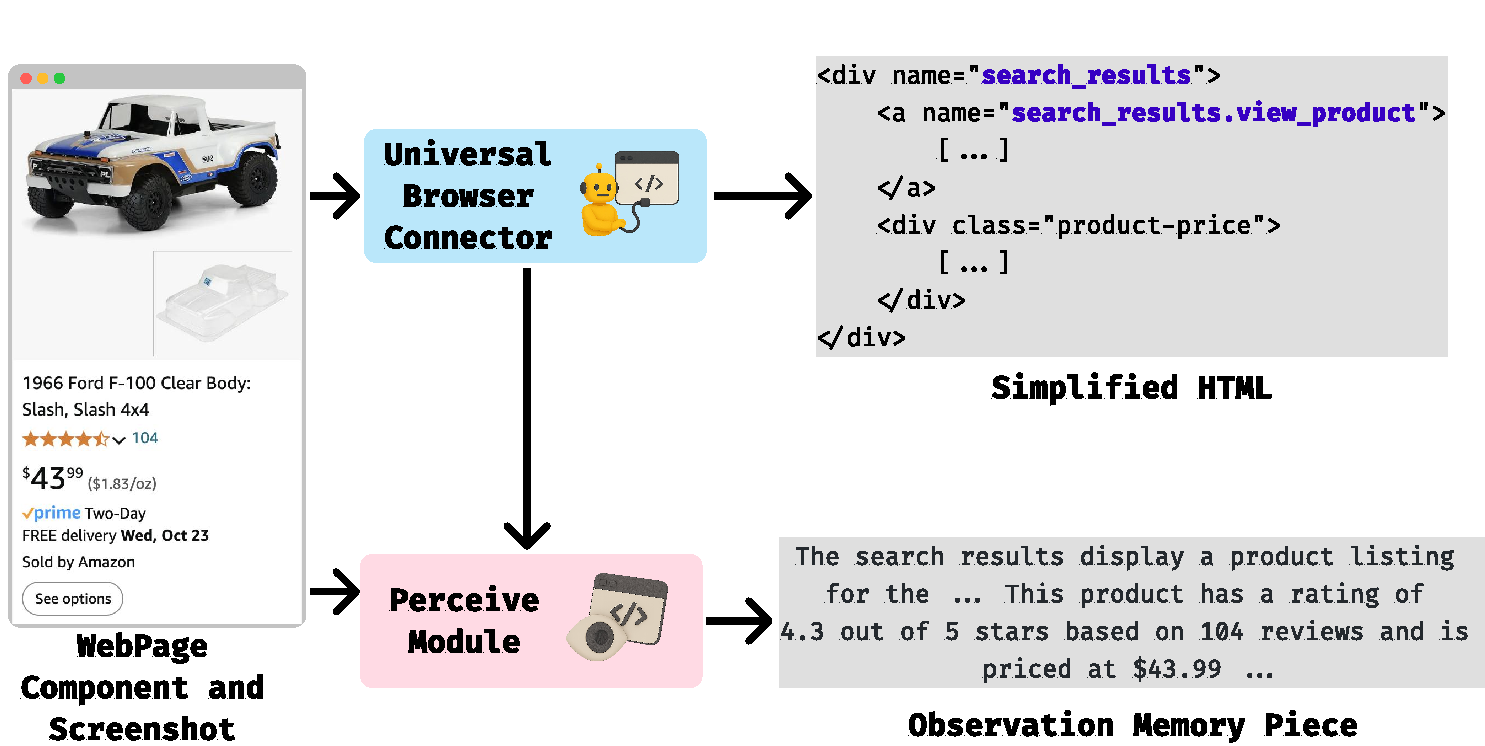
\includegraphics[width=\linewidth]{perception-demo.pdf}
    \caption{Universal Browser Connector}
  \end{figure}
\end{frame}

\begin{frame}{Generalizability}
  \begin{outline}
    \1 The agent is designed to be generalizable to different websites and tasks
    \1 Rufus: \url{https://broadcast.amazon.com/videos/1685504}
    \1 Customer Service Agent: \url{https://broadcast.amazon.com/videos/1685507}
    \1 AC3: \url{https://broadcast.amazon.com/videos/1769741}
  \end{outline}
\end{frame}

\begin{frame}[standout]
  Questions?
\end{frame}

\end{document}